% Copyright 2004 by Till Tantau <tantau@users.sourceforge.net>.
%
% In principle, this file can be redistributed and/or modified under
% the terms of the GNU Public License, version 2.
%
% However, this file is supposed to be a template to be modified
% for your own needs. For this reason, if you use this file as a
% template and not specifically distribute it as part of a another
% package/program, I grant the extra permission to freely copy and
% modify this file as you see fit and even to delete this copyright
% notice. 

\documentclass{beamer}

% There are many different themes available for Beamer. A comprehensive
% list with examples is given here:
% http://deic.uab.es/~iblanes/beamer_gallery/index_by_theme.html
% You can uncomment the themes below if you would like to use a different
% one:
%\usetheme{AnnArbor}
%\usetheme{Antibes}
%\usetheme{Bergen}
%\usetheme{Berkeley}
%\usetheme{Berlin}
%\usetheme{Boadilla}
%\usetheme{boxes}
%\usetheme{CambridgeUS}
%\usetheme{Copenhagen}
%\usetheme{Darmstadt}
\usetheme{default}
%\usetheme{Frankfurt}
%\usetheme{Goettingen}
%\usetheme{Hannover}
%\usetheme{Ilmenau}
%\usetheme{JuanLesPins}
%\usetheme{Luebeck}
%\usetheme{Madrid}
%\usetheme{Malmoe}
%\usetheme{Marburg}
%\usetheme{Montpellier}
%\usetheme{PaloAlto}
%\usetheme{Pittsburgh}
%\usetheme{Rochester}
%\usetheme{Singapore}
%\usetheme{Szeged}
%\usetheme{Warsaw}

\usepackage[serbian]{babel}


\title{Pomerač faze reflektivnog tipa}

% A subtitle is optional and this may be deleted
\subtitle{[13M071MMT] - Milimetarski talasi}

\author{student Aleksandar Vuković}
% - Give the names in the same order as the appear in the paper.
% - Use the \inst{?} command only if the authors have different
%   affiliation.

\institute[Univerzitet u Beogradu] % (optional, but mostly needed)
{
  Univerzitet u Beogradu \\
  Elektrotehnički fakultet
}
% - Use the \inst command only if there are several affiliations.
% - Keep it simple, no one is interested in your street address.

\date{22. 7. 2019.}
% - Either use conference name or its abbreviation.
% - Not really informative to the audience, more for people (including
%   yourself) who are reading the slides online

\subject{[13M071MMT] - Milimetarski talasi}
% This is only inserted into the PDF information catalog. Can be left
% out. 

% If you have a file called "university-logo-filename.xxx", where xxx
% is a graphic format that can be processed by latex or pdflatex,
% resp., then you can add a logo as follows:

% \pgfdeclareimage[height=0.5cm]{university-logo}{university-logo-filename}
% \logo{\pgfuseimage{university-logo}}

% Delete this, if you do not want the table of contents to pop up at
% the beginning of each subsection:
\AtBeginSubsection[]
{
  \begin{frame}<beamer>{Sadržaj}
    \tableofcontents[currentsection,currentsubsection]
  \end{frame}
}

% Let's get started
\begin{document}

\begin{frame}
  \titlepage
\end{frame}

% \begin{frame}{Outline}
%   \tableofcontents
%   % You might wish to add the option [pausesections]
% \end{frame}

% Section and subsections will appear in the presentation overview
% and table of contents.
\section{Uvod}

% \subsection{First Subsection}

\begin{frame}{Uvod}{Sadržaj prezentacije}
  \begin{itemize}
  \item {
    Pomerač faze reflektivnog tipa sa 360$^o$ opsegom za \textit{smart} antenske sisteme za C-opseg u 0.6 $\mu$m GaAs MESFET tehnologiji (2002)
  }

  \item {
    16-elementni fazirani niz kao prijemnik za opseg oko 60 GHz u IBM 0.12 $\mu$m SiGe BiCMOS tehnologiji (2011)
  }

  \item {
    Pomerač faze reflektivnog tipa sa konstantnim gubicima za oko 24 GHz u 0.18 $\mu$m CMOS tehnologiji (2015)
  }
  \end{itemize}
\end{frame}

% \item {
%     Ultracompact Reflective-Type Phase Shifter MMIC at C-Band With 360 Phase-Control Range for Smart Antenna Combining (2002)
%   }

%   \item {
%     A Fully-Integrated 16-Element Phased-Array Receiver in SiGe BiCMOS for 60-GHz Communications (2011)
%   }

%   \item {
%     A 24 GHz reflective-type phase shifter with constant loss in 0.18 $\mu$m CMOS technology (2015)
%   }

\section{Prvi rad}

% first paper first frame

\begin{frame}
  \frametitle{Prijemnik}
  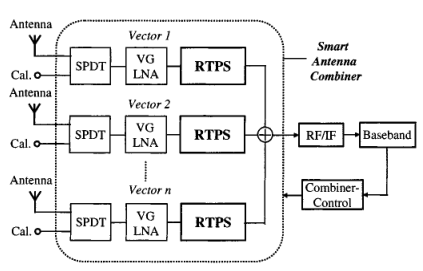
\includegraphics[width=0.7\linewidth]{ellinger_receiver.png}
\end{frame}

% first paper second frame

% first paper third frame


\begin{frame}

\begin{center}
\begin{tabular}{ | c | c | }
  \hline
  učestanost & 24 GHz \\
  \hline 
  opseg faznog pomeraja & 185$^o$ \\  
  \hline
  maksimalni gubici & 10.7 dB \\
  \hline
  varijacija gubitaka & 0 \\
  \hline
  S11 & $<$ 15 dB \\
  \hline
  potrošnja & 0 \\
  \hline
  površina na čipu & 0.7 mm$^2$  \\  
  \hline
\end{tabular}
\end{center}
\end{frame}

\section{Drugi rad}

% You can reveal the parts of a slide one at a time
% with the \pause command:

% second paper first frame

\begin{frame}
\frametitle{\textit{Beamforming} predajnik}
\begin{columns}
  \begin{column}{0.5\textwidth}
    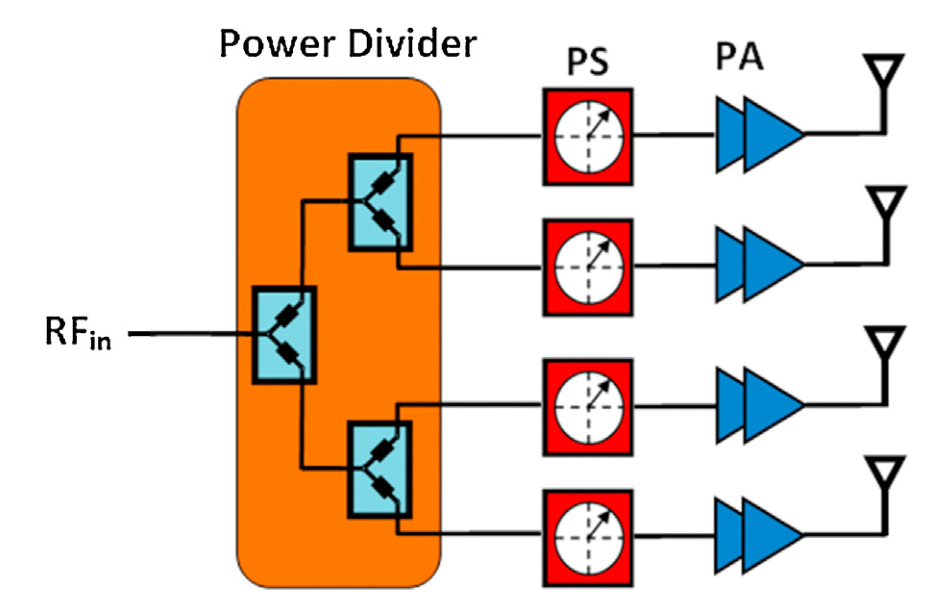
\includegraphics[width=\linewidth]{beam_forming_transmitter.png}
  \end{column}
  \begin{column}{0.5\textwidth}
    Specifikacije:
    \begin{itemize}
      \item varijacija slabljenja u odnosu na fazni pomeraj
      \item potrošnja 
    \end{itemize}
  \end{column}
\end{columns}
\end{frame}

% second paper second frame

\begin{frame}
\frametitle{Hibridni sprežnjak}
\begin{columns}
\begin{column}{0.5\textwidth}
   some text here some text here some text here some text here some text here
\end{column}
\begin{column}{0.5\textwidth}  
    \begin{center}
     %%%%% this is a minipage, so \textwidth is already adjusted to the size of the column
     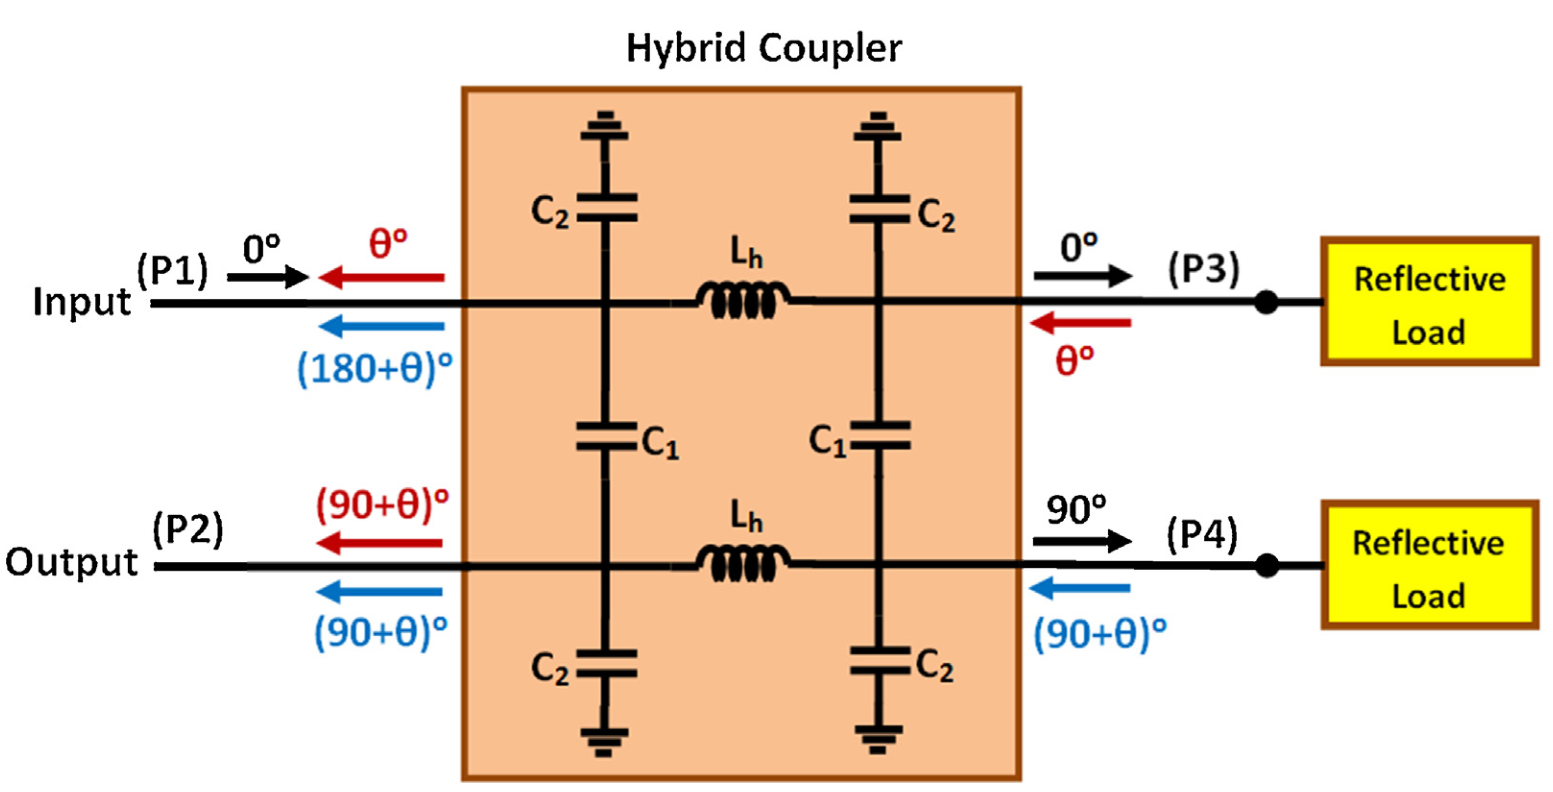
\includegraphics[width=\textwidth]{hybrid_coupler.png}
     \end{center}
\end{column}
\end{columns}
\end{frame}



\begin{frame}
\frametitle{Rezultati simulacija}
\begin{columns}
  \begin{column}{0.5\textwidth}
    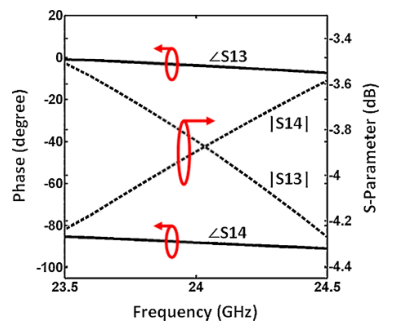
\includegraphics[width=\textwidth]{sparam_hybrid_coupler.png}
  \end{column}
  \begin{column}{0.5\textwidth}
    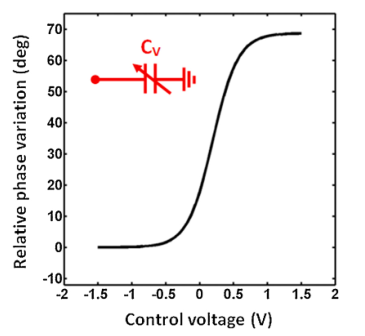
\includegraphics[width=\textwidth]{phase_variation_across_control_voltage.png}
  \end{column}
\end{columns}
\end{frame}

\begin{frame}
\frametitle{AMOS varaktor}
% \begin{columns}
  % \begin{column}{0.5\textwidth}
    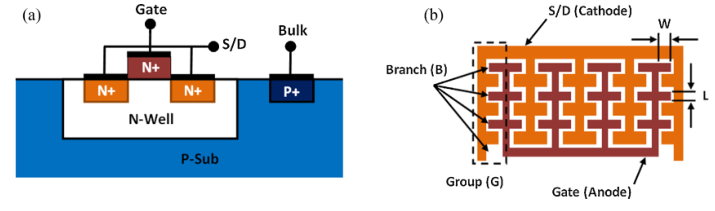
\includegraphics[width=\textwidth]{amos_varactor.png}
  % \end{column}
  % \begin{column}{0.5\textwidth}
    Varaktor ima opseg za podešavanje of 80 fF do 240 fF, sa prosečnom parazitnom otpornošću od 1.5 $\Omega$ i prosečnom parazitnom kapacitivnošću 8 pH.
  % \end{column}

% \end{columns}
\end{frame}

% \begin{frame}
% \frametitle{}
%       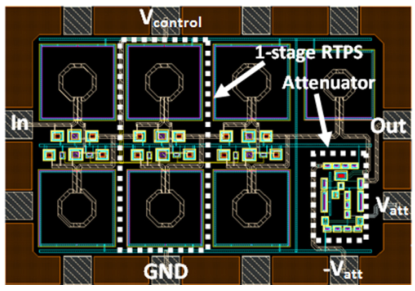
\includegraphics[width=\textwidth]{rtps_layout.png}

% \end{frame}


\begin{frame}
  \frametitle{}
  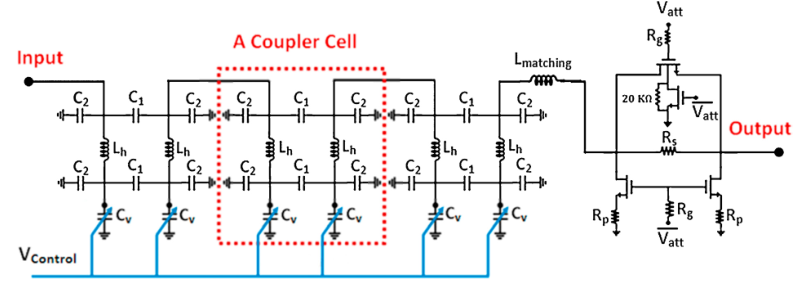
\includegraphics[width=\textwidth]{proposed_sch_coupler_cells_attenuator.png}

\end{frame}


\begin{frame}
\frametitle{Rezultati simulacija}
\begin{columns}
  \begin{column}{0.5\textwidth}
    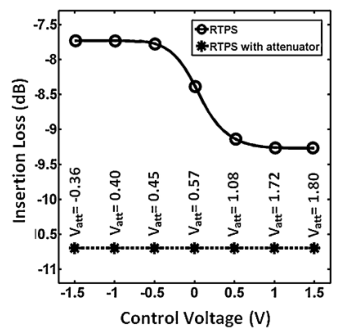
\includegraphics[width=\textwidth]{insertion_loss_w_wo_att.png}
  \end{column}
  \begin{column}{0.5\textwidth}
    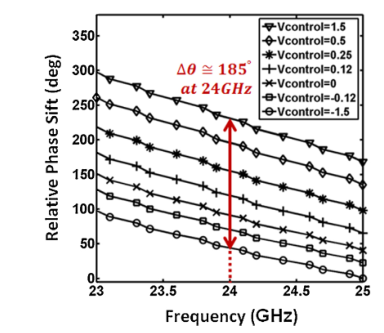
\includegraphics[width=\textwidth]{phase_shift_range.png}
  \end{column}
\end{columns}
\end{frame}


\begin{frame}
\frametitle{Rezultati simulacija i lejaut}
\begin{columns}
  \begin{column}{0.5\textwidth}
    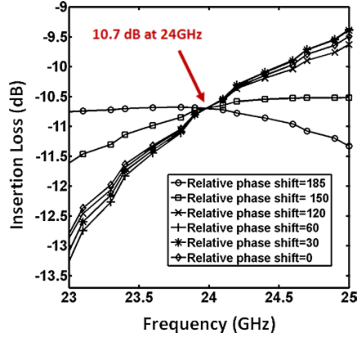
\includegraphics[width=\textwidth]{insertion_loss_variation.png}
  \end{column}
  \begin{column}{0.5\textwidth}
    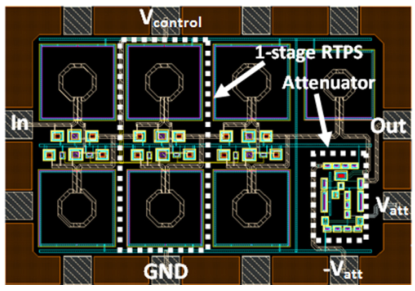
\includegraphics[width=\textwidth]{rtps_layout.png}
  \end{column}
\end{columns}
\end{frame}


\begin{frame}
\frametitle{Pregled rezultata i naziv rada sa autorima}
\begin{center}
\begin{tabular}{ | c | c | }
  \hline
  učestanost & 24 GHz \\
  \hline 
  opseg faznog pomeraja & 185$^o$ \\  
  \hline
  maksimalni gubici & 10.7 dB \\
  \hline
  varijacija gubitaka & 0 \\
  \hline
  S11 & $<$ 15 dB \\
  \hline
  potrošnja & 0 \\
  \hline
  površina na čipu & 0.7 mm$^2$  \\  
  \hline
\end{tabular}
\end{center}
\end{frame}

\section{Treći rad}

\begin{frame}

\end{frame}

% \begin{frame}{Pomerač faze reflektivnog tipa}
%   \begin{columns}
%     \begin{column}{width=0.5\textwidth}
%     pt
%       % \begin{itemize}
%       %   \item 1
%       %   \item 2
%       % \end{itemize}
%     \end{column}
%     \begin{column}{width=0.5\textwidth}
%         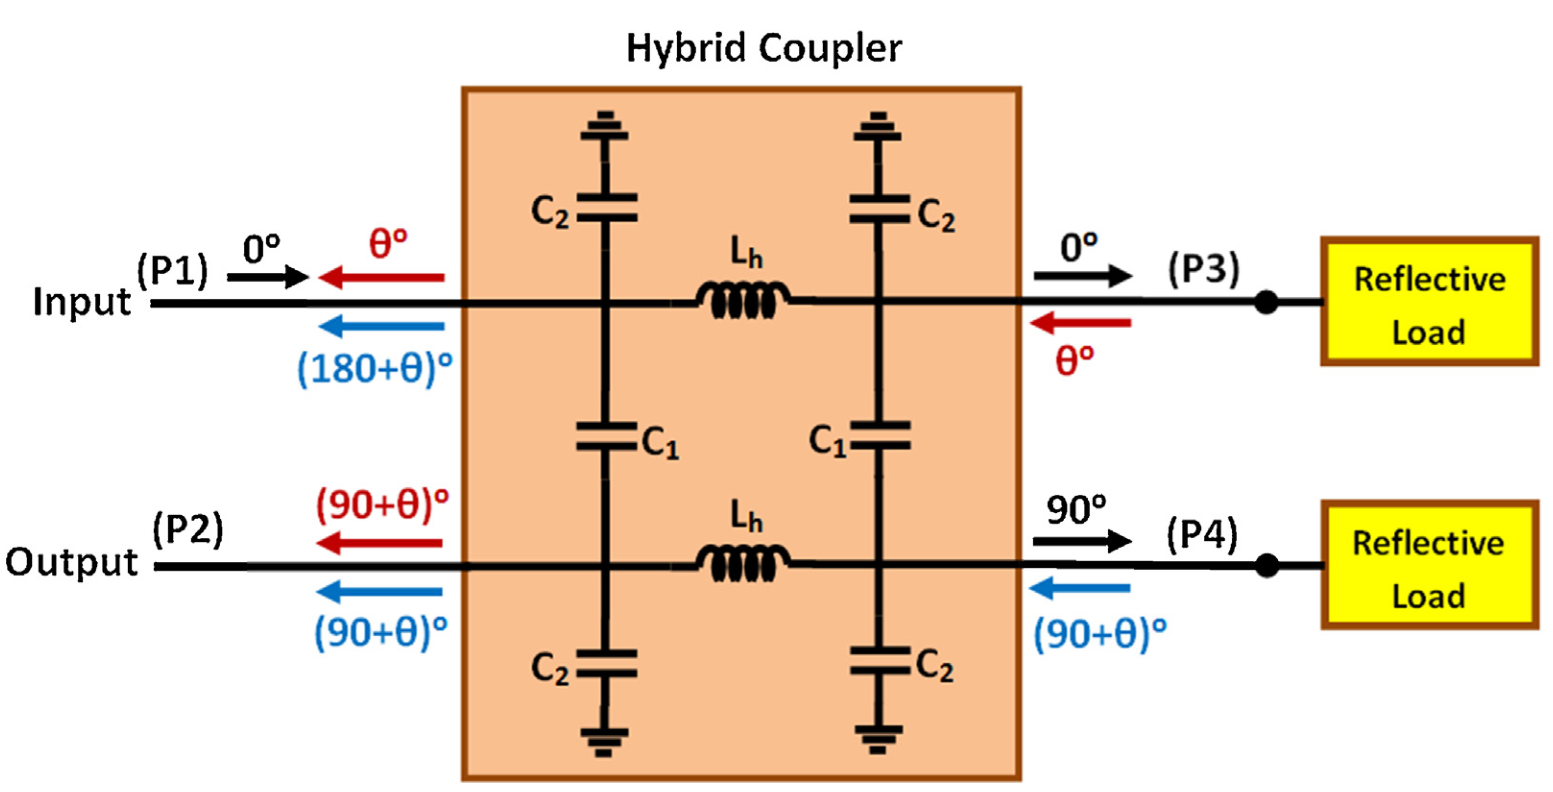
\includegraphics[width=\linewidth]{hybrid_coupler.png}
%     \end{column}
%   \end{columns}
  
% \end{frame}

\begin{frame}
\frametitle{Poređenje bežičnih linkova antenskog elementa i antenskog niza}
  \begin{figure}[!htbp]
    \centering
    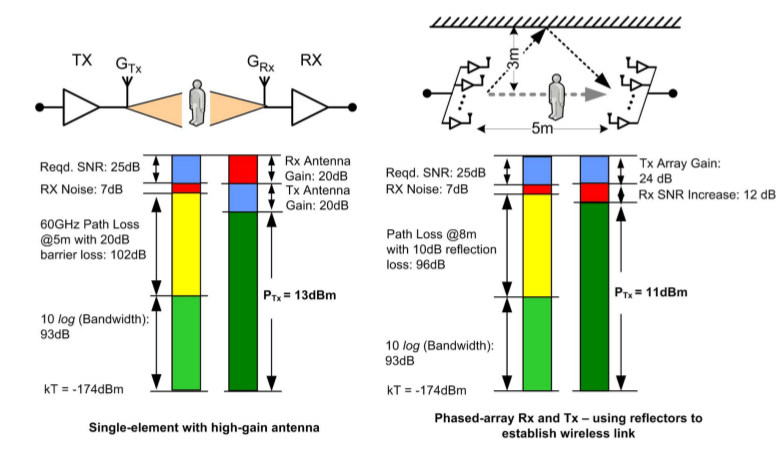
\includegraphics[width=\linewidth]{link_single_element_vs_phased-array@60GHz.png}
    \label{fig:element_vs_array}
  \end{figure}
\end{frame}

% Ovde frejm sa pričom o SNR faziranog niza u poređenju sa jednim antenskim elementom


\begin{frame}
  \frametitle{Arhitektura prijemnika}
  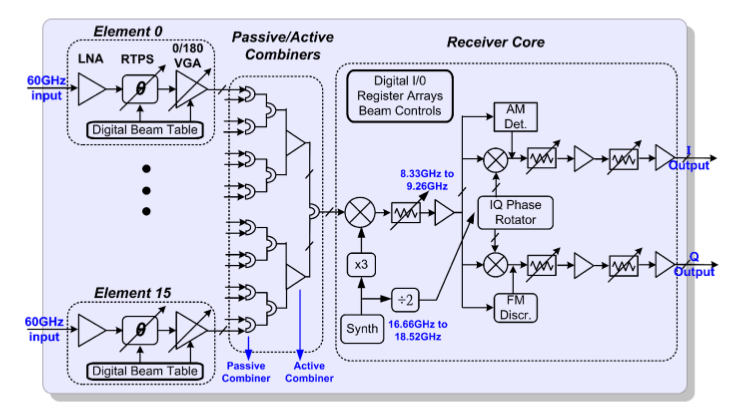
\includegraphics[width=\linewidth]{rx-arch-freq-plan.png}
\end{frame}

\begin{frame}
\frametitle{\textit{Gysel} kombajner}
  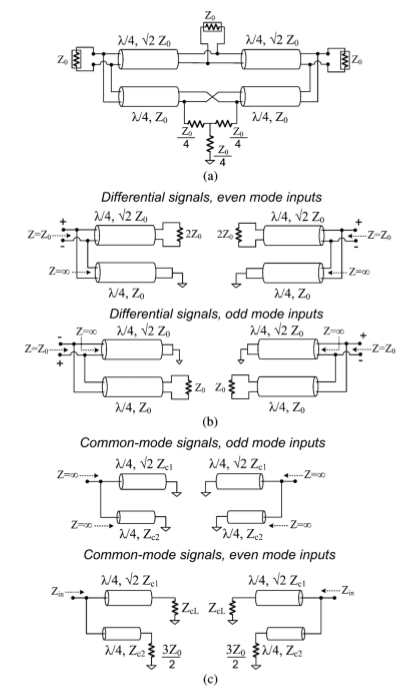
\includegraphics[width=0.45\linewidth]{Gysel-power-combiner.png}
\end{frame}


\begin{frame}
\frametitle{Lejaut !?}
  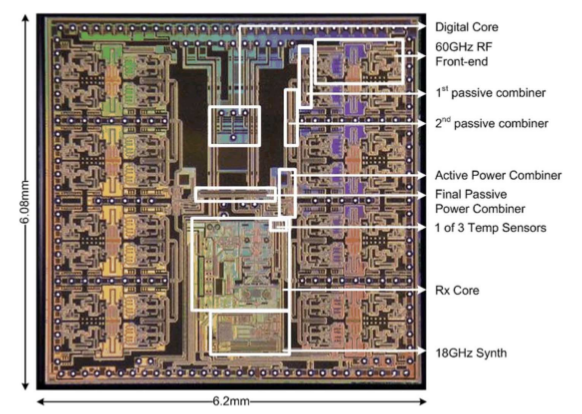
\includegraphics[width=\linewidth]{layout60GHz-IBM.png}
\end{frame}





% \begin{frame}{Second Slide Title}
%   \begin{itemize}
%   \item {
%     First item.
%     \pause % The slide will pause after showing the first item
%   }
%   \item {   
%     Second item.
%   }
%   % You can also specify when the content should appear
%   % by using <n->:
%   \item<3-> {
%     Third item.
%   }
%   \item<4-> {
%     Fourth item.
%   }
%   % or you can use the \uncover command to reveal general
%   % content (not just \items):
%   \item<5-> {
%     Fifth item. \uncover<6->{Extra text in the fifth item.}
%   }
%   \end{itemize}
% \end{frame}

% \section{Second Main Section}

% \subsection{Another Subsection}

% \begin{frame}{Blocks}
% \begin{block}{Block Title}
% You can also highlight sections of your presentation in a block, with it's own title
% \end{block}
% \begin{theorem}
% There are separate environments for theorems, examples, definitions and proofs.
% \end{theorem}
% \begin{example}
% Here is an example of an example block.
% \end{example}
% \end{frame}

% Placing a * after \section means it will not show in the
% outline or table of contents.
\section*{Summary}

\begin{frame}{Summary}
  \begin{itemize}
  \item
    The \alert{first main message} of your talk in one or two lines.
  \item
    The \alert{second main message} of your talk in one or two lines.
  \item
    Perhaps a \alert{third message}, but not more than that.
  \end{itemize}
  
  \begin{itemize}
  \item
    Outlook
    \begin{itemize}
    \item
      Something you haven't solved.
    \item
      Something else you haven't solved.
    \end{itemize}
  \end{itemize}
\end{frame}



% All of the following is optional and typically not needed. 
\appendix
\section<presentation>*{\appendixname}
\subsection<presentation>*{For Further Reading}

\begin{frame}[allowframebreaks]
  \frametitle<presentation>{For Further Reading}
    
  \begin{thebibliography}{10}
    
  \beamertemplatebookbibitems
  % Start with overview books.

  \bibitem{Author1990}
    A.~Author.
    \newblock {\em Handbook of Everything}.
    \newblock Some Press, 1990.
 
    
  \beamertemplatearticlebibitems
  % Followed by interesting articles. Keep the list short. 

  \bibitem{Someone2000}
    S.~Someone.
    \newblock On this and that.
    \newblock {\em Journal of This and That}, 2(1):50--100,
    2000.
  \end{thebibliography}
\end{frame}

\end{document}
